\documentclass[12pt,reqno,final,pdftex]{amsart}\usepackage[]{graphicx}\usepackage[]{color}
%% maxwidth is the original width if it is less than linewidth
%% otherwise use linewidth (to make sure the graphics do not exceed the margin)
\makeatletter
\def\maxwidth{ %
  \ifdim\Gin@nat@width>\linewidth
    \linewidth
  \else
    \Gin@nat@width
  \fi
}
\makeatother

\definecolor{fgcolor}{rgb}{0.345, 0.345, 0.345}
\newcommand{\hlnum}[1]{\textcolor[rgb]{0.686,0.059,0.569}{#1}}%
\newcommand{\hlstr}[1]{\textcolor[rgb]{0.192,0.494,0.8}{#1}}%
\newcommand{\hlcom}[1]{\textcolor[rgb]{0.678,0.584,0.686}{\textit{#1}}}%
\newcommand{\hlopt}[1]{\textcolor[rgb]{0,0,0}{#1}}%
\newcommand{\hlstd}[1]{\textcolor[rgb]{0.345,0.345,0.345}{#1}}%
\newcommand{\hlkwa}[1]{\textcolor[rgb]{0.161,0.373,0.58}{\textbf{#1}}}%
\newcommand{\hlkwb}[1]{\textcolor[rgb]{0.69,0.353,0.396}{#1}}%
\newcommand{\hlkwc}[1]{\textcolor[rgb]{0.333,0.667,0.333}{#1}}%
\newcommand{\hlkwd}[1]{\textcolor[rgb]{0.737,0.353,0.396}{\textbf{#1}}}%
\let\hlipl\hlkwb

\usepackage{framed}
\makeatletter
\newenvironment{kframe}{%
 \def\at@end@of@kframe{}%
 \ifinner\ifhmode%
  \def\at@end@of@kframe{\end{minipage}}%
  \begin{minipage}{\columnwidth}%
 \fi\fi%
 \def\FrameCommand##1{\hskip\@totalleftmargin \hskip-\fboxsep
 \colorbox{shadecolor}{##1}\hskip-\fboxsep
     % There is no \\@totalrightmargin, so:
     \hskip-\linewidth \hskip-\@totalleftmargin \hskip\columnwidth}%
 \MakeFramed {\advance\hsize-\width
   \@totalleftmargin\z@ \linewidth\hsize
   \@setminipage}}%
 {\par\unskip\endMakeFramed%
 \at@end@of@kframe}
\makeatother

\definecolor{shadecolor}{rgb}{.97, .97, .97}
\definecolor{messagecolor}{rgb}{0, 0, 0}
\definecolor{warningcolor}{rgb}{1, 0, 1}
\definecolor{errorcolor}{rgb}{1, 0, 0}
\newenvironment{knitrout}{}{} % an empty environment to be redefined in TeX

\usepackage{alltt}
%% DO NOT DELETE OR CHANGE THE FOLLOWING TWO LINES!
%% $Revision$
%% $Date$
\usepackage[round,sort,elide]{natbib}
\usepackage{graphicx}
\usepackage{times}
\usepackage{rotating}
\usepackage{subfig}
\usepackage{color}
\newcommand{\aak}[1]{\textcolor{cyan}{#1}}
\newcommand{\mab}[1]{\textcolor{red}{#1}}
\newcommand{\cec}[1]{\textcolor{blue}{#1}}

\setlength{\textwidth}{6.25in}
\setlength{\textheight}{8.75in}
\setlength{\evensidemargin}{0in}
\setlength{\oddsidemargin}{0in}
\setlength{\topmargin}{-.35in}
\setlength{\parskip}{.1in}
\setlength{\parindent}{0.3in}

%% cleveref must be last loaded package
\usepackage[sort&compress]{cleveref}
\newcommand{\crefrangeconjunction}{--}
\crefname{figure}{Fig.}{Figs.}
\Crefname{figure}{Fig.}{Figs.}
\crefname{table}{Table}{Tables}
\Crefname{table}{Tab.}{Tables}
\crefname{equation}{Eq.}{Eqs.}
\Crefname{equation}{Eq.}{Eqs.}
\crefname{appendix}{Appendix}{Appendices}
\Crefname{appendix}{Appendix}{Appendices}
\creflabelformat{equation}{#2#1#3}

\theoremstyle{plain}
\newtheorem{thm}{Theorem}
\newtheorem{corol}[thm]{Corollary}
\newtheorem{prop}[thm]{Proposition}
\newtheorem{lemma}[thm]{Lemma}
\newtheorem{defn}[thm]{Definition}
\newtheorem{hyp}[thm]{Hypothesis}
\newtheorem{example}[thm]{Example}
\newtheorem{conj}[thm]{Conjecture}
\newtheorem{algorithm}[thm]{Algorithm}
\newtheorem{remark}{Remark}
\renewcommand\thethm{\arabic{thm}}
\renewcommand{\theremark}{}

\numberwithin{equation}{part}
\renewcommand\theequation{\arabic{equation}}
\renewcommand\thesection{\arabic{section}}
\renewcommand\thesubsection{\thesection.\arabic{subsection}}
\renewcommand\thefigure{\arabic{figure}}
\renewcommand\thetable{\arabic{table}}
\renewcommand\thefootnote{\arabic{footnote}}

\newcommand\scinot[2]{$#1 \times 10^{#2}$}
\newcommand{\code}[1]{\texttt{#1}}
\newcommand{\pkg}[1]{\textsf{#1}}
\newcommand{\dlta}[1]{{\Delta}{#1}}
\newcommand{\Prob}[1]{\mathbb{P}\left[#1\right]}
\newcommand{\Expect}[1]{\mathbb{E}\left[#1\right]}
\newcommand{\Var}[1]{\mathrm{Var}\left[#1\right]}
\newcommand{\dd}[1]{\mathrm{d}{#1}}
\newcommand{\citetpos}[1]{\citeauthor{#1}'s \citeyearpar{#1}}
\IfFileExists{upquote.sty}{\usepackage{upquote}}{}
\begin{document}






The first thing I want to consider is a comparison of two methods of simulating a GEM.
The first is the classic GEM, which chooses an individual at random, uses a Monte Carlo algorithm to determine what happens to it based on the individual's traits, and then advances time a random amount based on the total rate of events for that individual.
The second method modifies the algorithm by creating the ``wheel of fortune'' using the rates for every individual in the population, and then using the Monte Carlo algorithm to choose both an individual and an event from a single ``spin'' of the wheel.
Obviously, time will advance much more slowly in the second model because the timestep is chosen using the code exp(-1/sum(events))/sum(events): since the second method sums across all events (births and deaths) for every individual in the population, the denominator is a very large number in the second method.

Fig. \ref{fig:originalGEM} shows the population and trait dynamics for the original GEM method with increasing carrying capacity (the different columns) and initial conditions of $N(0) = 5$, mean trait of 1.8, trait CV of 0.3, and heritability of 0.75.

Fig. \ref{fig:manysliceGEM} shows the same

\begin{knitrout}\scriptsize
\definecolor{shadecolor}{rgb}{0.969, 0.969, 0.969}\color{fgcolor}\begin{figure}

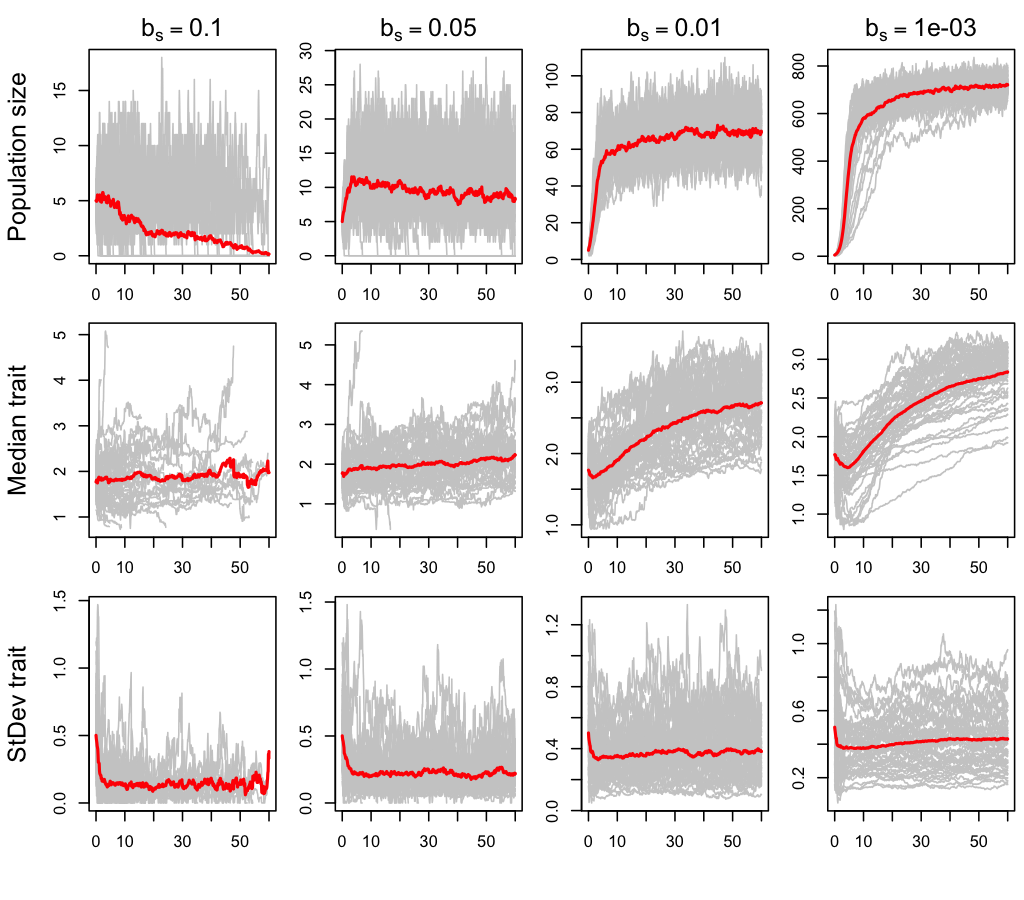
\includegraphics[width=\linewidth]{figure/originalGEM-1} \hfill{}

\caption[Population and trait dynamics for the original GEM]{Population and trait dynamics for the original GEM.}\label{fig:originalGEM}
\end{figure}


\end{knitrout}

\begin{knitrout}\scriptsize
\definecolor{shadecolor}{rgb}{0.969, 0.969, 0.969}\color{fgcolor}\begin{figure}

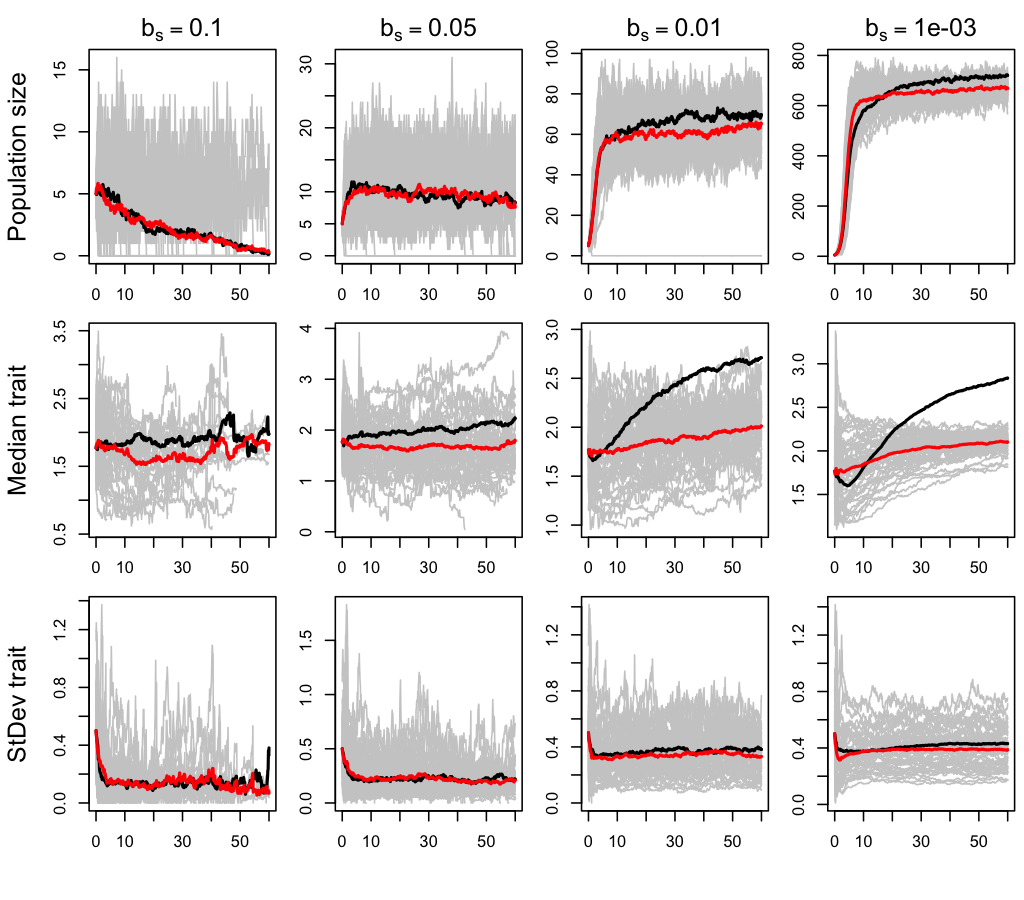
\includegraphics[width=\linewidth]{figure/manysliceGEM-1} \hfill{}

\caption[Population and trait dynamics for the many-slice GEM]{Population and trait dynamics for the many-slice GEM. The black line shows the mean dynamics from the original GEM simulations above.}\label{fig:manysliceGEM}
\end{figure}


\end{knitrout}


\end{document}
